\documentclass{beamer}

\usepackage{listings}
\lstset{ % General setup for the package
    language=VHDL,
    numbers=left,
    frame=tb,
    tabsize=4,
    columns=fixed,
    showstringspaces=false,
    showtabs=false,
    keepspaces,
    commentstyle=\color{brown},
    keywordstyle=\color{blue},
    stringstyle=\color{red},
    title=\lstname,
    basicstyle = \tiny,
    breaklines=true,
    }

\usecolortheme{beaver}
\setbeamertemplate{navigation symbols}{}
\setbeamertemplate{footline}[frame number]

\title{Mandelbrot Pong}
\subtitle{EE-334 Digital systems design}
\author[Thür, Mheni] 
	{Simon~Thür \and Lokman~Mheni}
\institute[EPFL]{EPFL SEL-BA5}
\subject{Digital systems design}

\begin{document}
\frame {
    \titlepage
}

\begin{frame}
    \frametitle{Table of Contents}
    \tableofcontents[currentsection]
\end{frame}


\section{VGA Controller}
\begin{frame}
    \sectionpage
\end{frame}

\begin{frame}
    \frametitle{VGA Controller}
    \begin{itemize}
        \item 2 Counters (x and y)
        \item Front porch, pulse, and backporch at Beginning of frame
        \item Edge detector on Vertical Sync (VSedgexSO corresponds to new frame)
        \item X,Y output corresponds to next color wanted
    \end{itemize}

    \begin{equation}
        \begin{split}
            X_{out} &= X{cntr} - (FP_{HS} + P_{HS} + BP_{HS})+1\\
            Y_{out} &= Y{cntr} - (FP_{VS} + P_{VS} + BP_{VS})
        \end{split}
    \end{equation}
\end{frame}


\section{Memory}
\begin{frame}
    \sectionpage
\end{frame}

\subsection{Coordinate mapping}
\begin{frame}[fragile]
    \frametitle{Memory}
    \framesubtitle{Coordinate mapping}
    \lstinputlisting[firstline=297,lastline=302]{../_00FINAL_PROJECT/src/mandelbrot_top.vhdl}
    firstline=297,lastline=302

\end{frame}


\subsection{Size constraints}
\begin{frame}
    \frametitle{Memory}
    \framesubtitle{Size constraints}
    \begin{alertblock}
        {16 bit constraint on memory address}
        Not enough space for 2 images (without reducing image resolution farther)
    \end{alertblock}
    \begin{figure}
        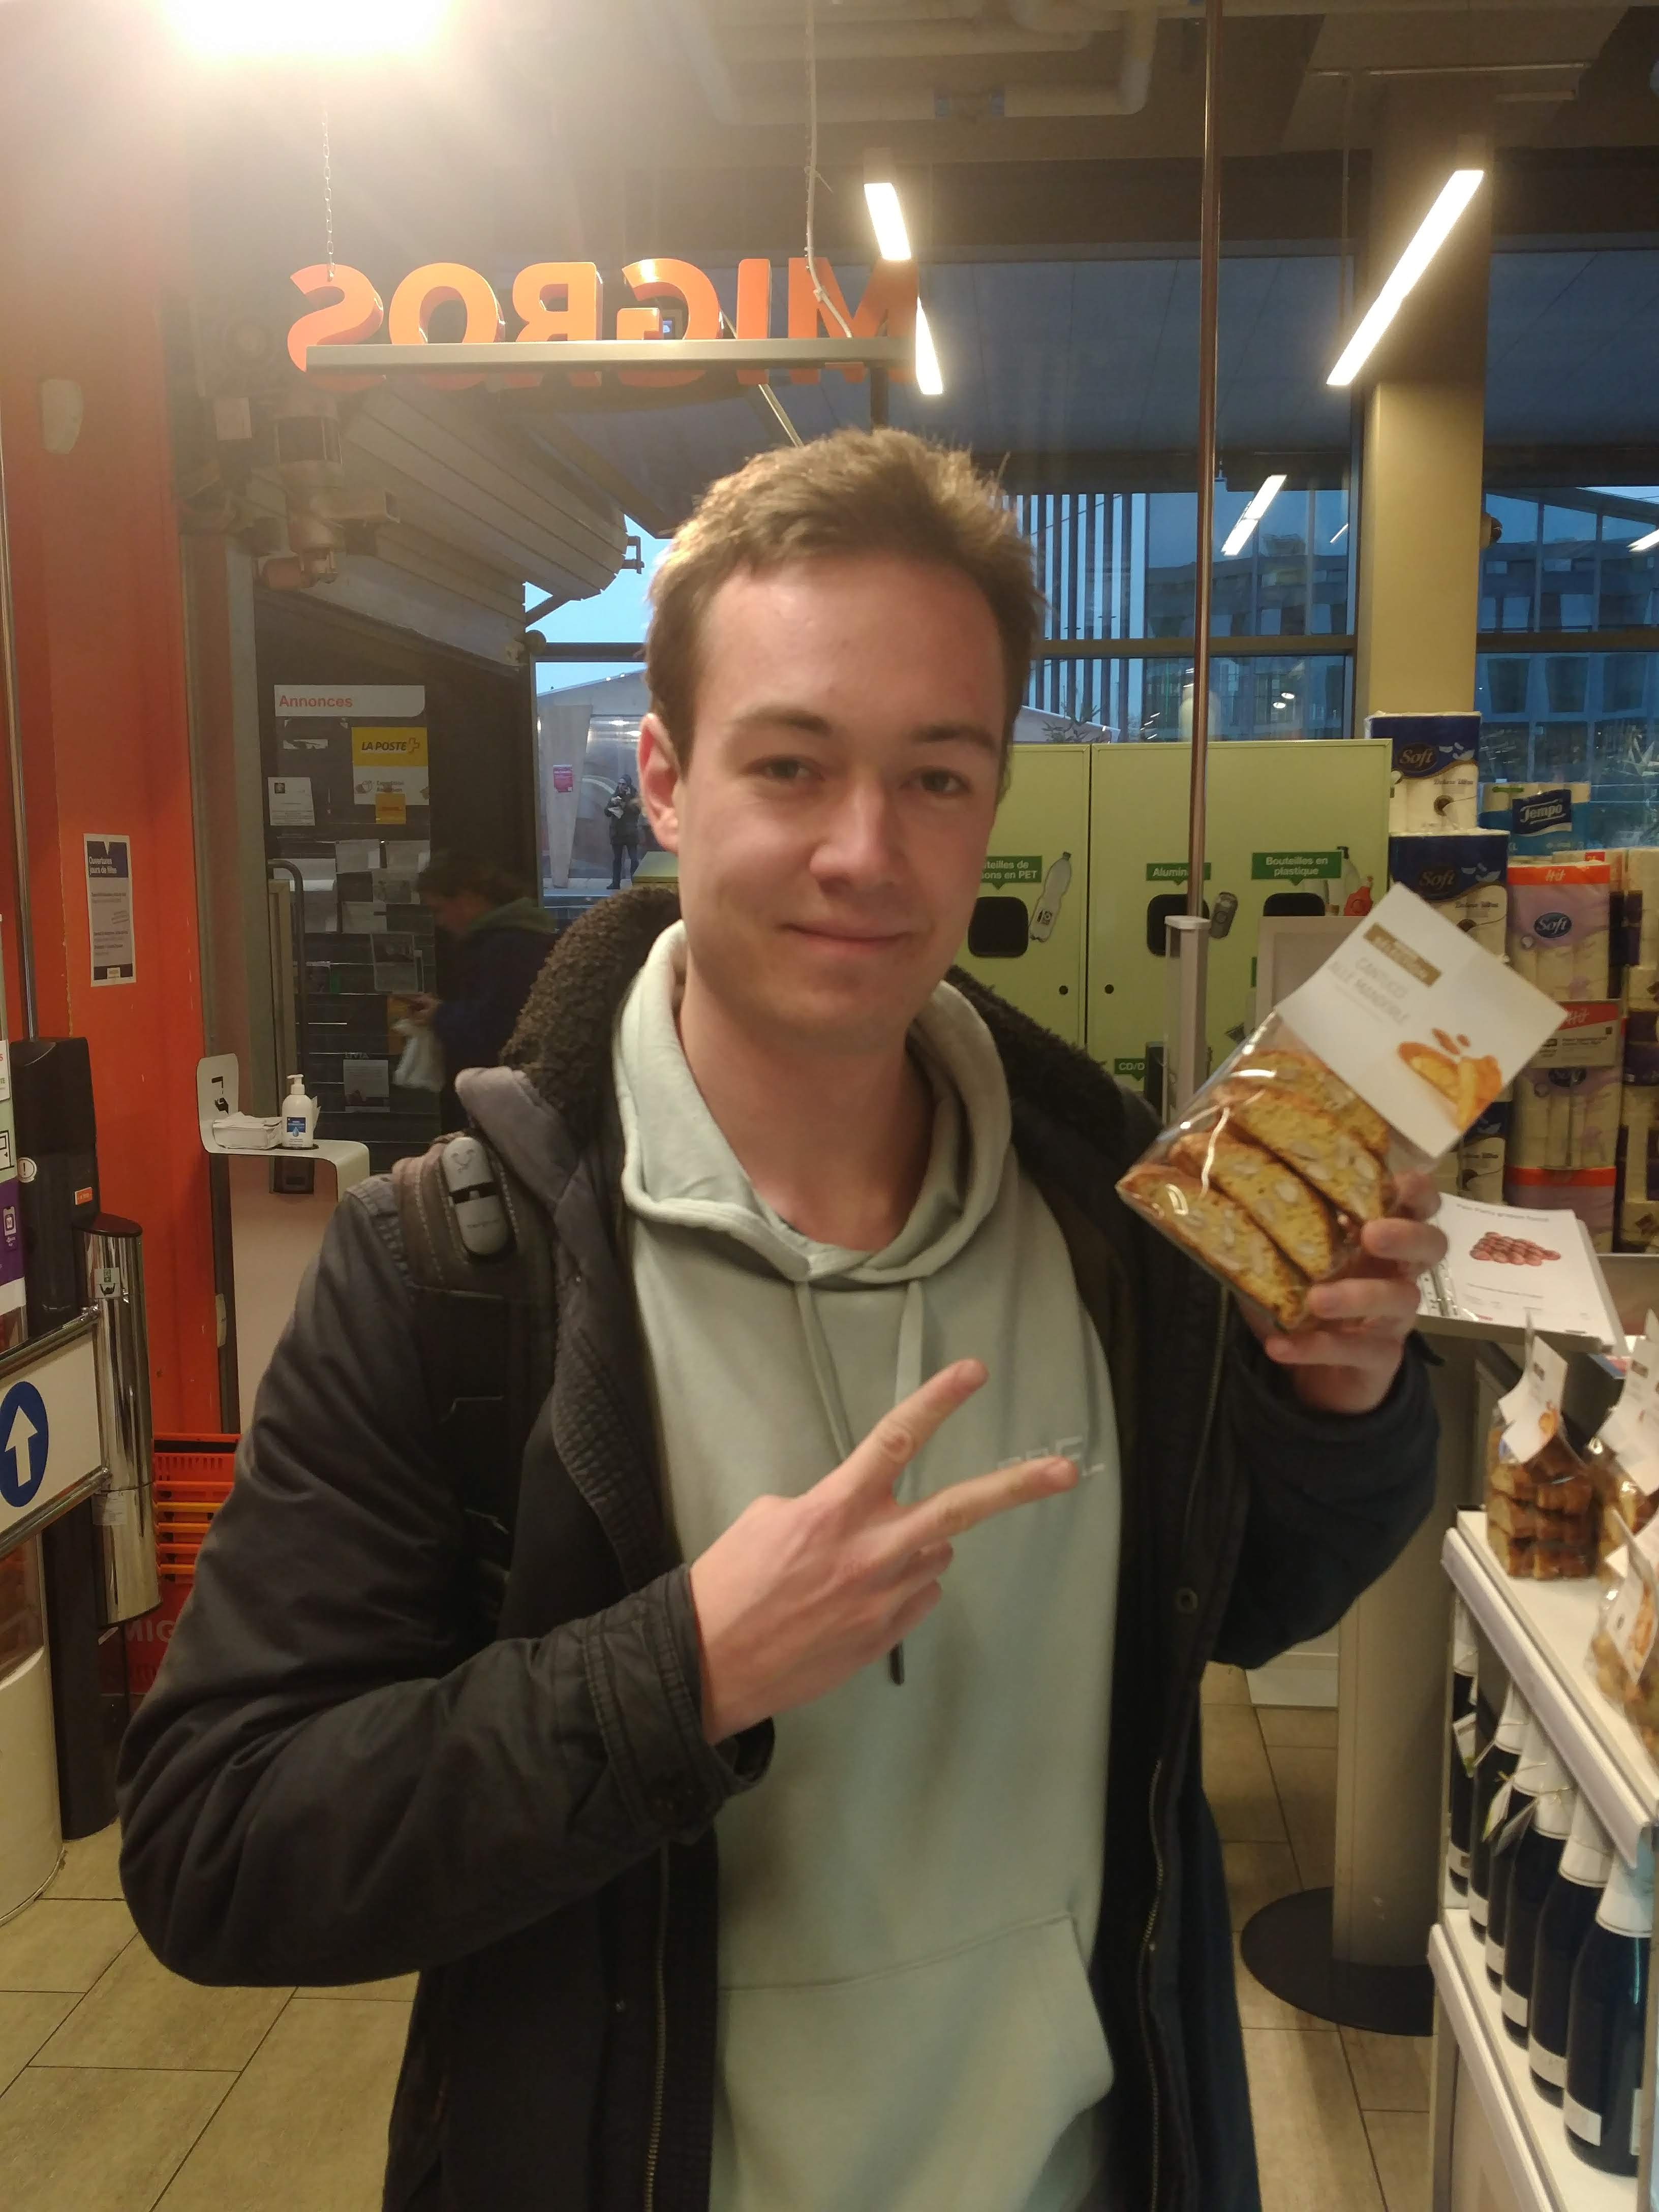
\includegraphics[width=.3\textwidth]{../_00FINAL_PROJECT/src/mandelbrot_und_so.jpg}
    \end{figure}
\end{frame}


\section{Pong}
\begin{frame}
    \sectionpage
\end{frame}

\subsection{Architecture}
\begin{frame}
    \frametitle{Pong}
    \framesubtitle{Control architecture}
    Elements used:
    \begin{itemize}
        \item Counters for X and Y of ball
        \item Counter for X of plate
        \item Control signals for game state
    \end{itemize}
\end{frame}

\subsection{State control}
\begin{frame}
    \frametitle{Pong}
    \framesubtitle{State control}
    \begin{alertblock}{No FSM!?}
        States are binary in nature,
        so we used binary signals to control the state:
        \begin{itemize}
            \item Direction left (not right)
            \item Direction up (not down)
            \item Game in progress (not paused)
        \end{itemize}
    \end{alertblock}
\end{frame}

\begin{frame}
    \frametitle{Pong}
    \framesubtitle{State control }
    \begin{block}{Game logic}
        Because our \emph{FSM} is only signals,
        boundry conditions mapped easily onto state transitions (change left-right/up-down or finish game).
    \end{block}
    \begin{block}{Random start position}
        We use the VGA-counter position to calculate a random position in the top half of the screen,
        as well as the starting direction (left-right)
    \end{block}
\end{frame}

\subsection{Sprite logic}
\begin{frame}[fragile]
    \frametitle{Pong}
    \framesubtitle{Sprite logic}
    We use a trivial process to overlay the ball onto the image by simple multiplexing the color output with logic:
    \lstinputlisting[firstline=319,lastline=338]{../_00FINAL_PROJECT/src/mandelbrot_top.vhdl}
    firstline=319, lastline=338
\end{frame}



\section{Mandelbrot generator}
\begin{frame}
    \sectionpage
\end{frame}

\subsection{Architecture}
\begin{frame}
    \frametitle{Mandelbrot}
    \framesubtitle{Architecture}
    \begin{block}{Iterative decomposition}
        Because the initial idea was having \textbf{two images},
        we initially aimed for \textbf{low space} usage.

        The further advantage of this approach is that it greatly \textbf{simplifies the control} of the calculation as it can be stopped before any overflow errors occur (as they might in an unrolled or pipelined architecture).
    \end{block}
\end{frame}

\subsection{Control path}
\begin{frame}
    \frametitle{Mandelbrot}
    \framesubtitle{Control path (base vesion)}
    \begin{block}{ Elements used for control}

        \begin{itemize}
            \item Counters for X and Y (for screen, 256x192)
            \item Count enable for X and Y
            \item Counter for iterations
            \item \emph{Done} logic block
        \end{itemize}
    \end{block}

    (In a second step more control is added for animations detailed in slide \ref{Animation})
\end{frame}


\begin{frame}
    \frametitle{Mandelbrot}
    \framesubtitle{Control - initial values}
    The initial values $c_r$ and $c_i$ are derived from the X and Y counter values.
    \begin{equation}
        \label{eq:startval}
        \begin{split}
            c_r &= c_{r_{inc}}  \cdot X + c_{r_0}\\
            c_i &= c_{i_{inc}}  \cdot Y + c_{i_0}\\
        \end{split}
    \end{equation}
    These get fed into $z_r$ and $z_i$ depending on the \emph{Done} signal.
    Equally X, Y, and iteration counters get updated on \emph{Done}.
\end{frame}

\subsection{Data path}
\begin{frame}
    \frametitle{Mandelbrot}
    \framesubtitle{Data path}
    Green the values of the first iteration, Red the fixed point position.
    \begin{figure}
        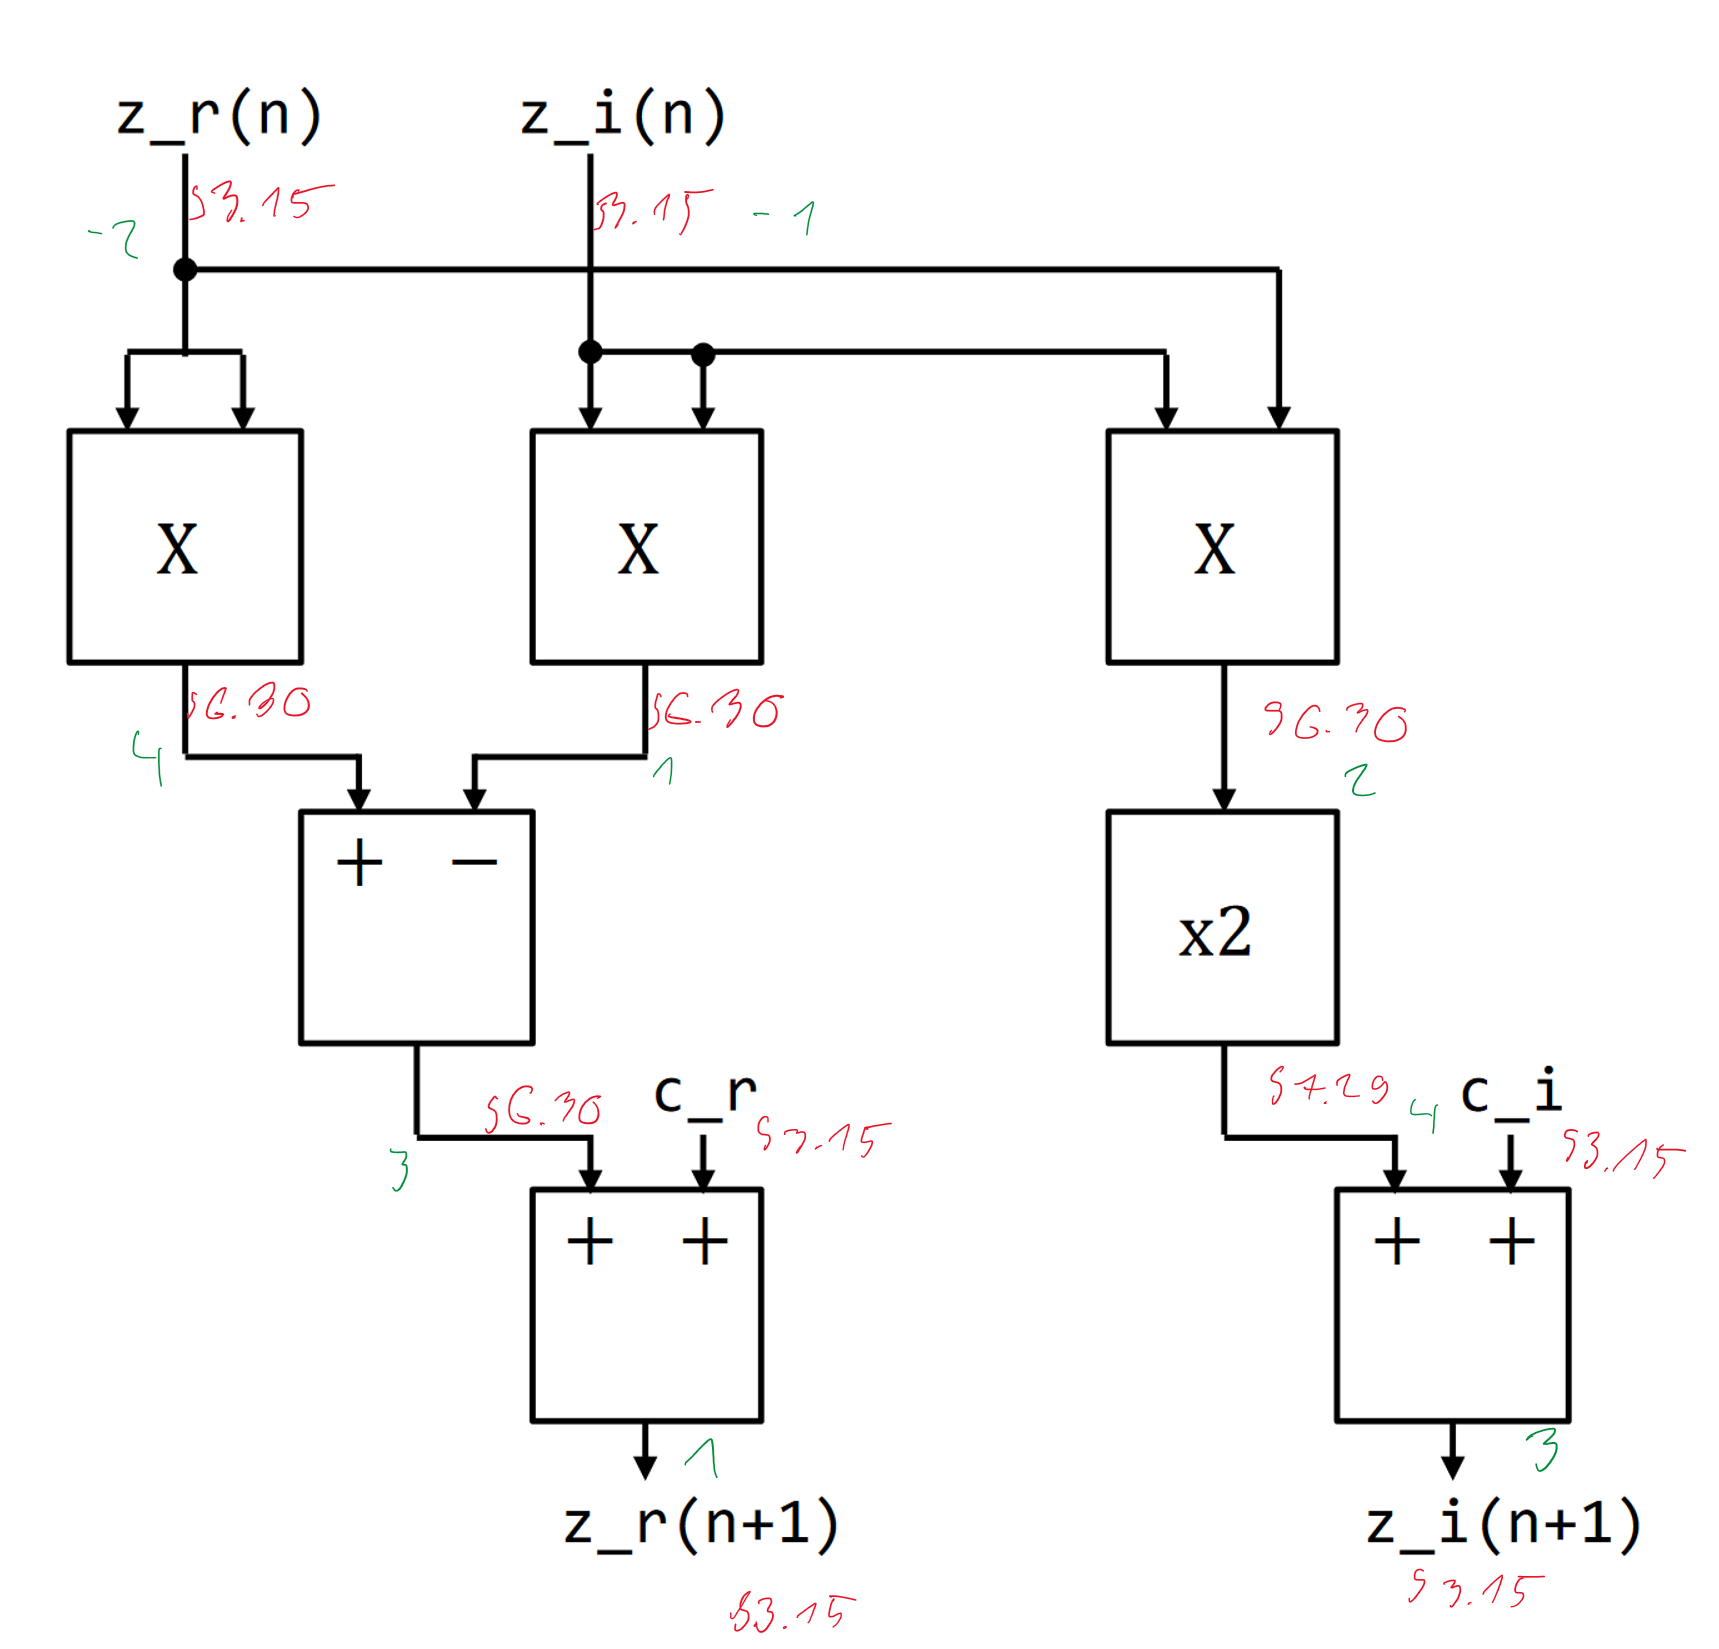
\includegraphics[width=.65\textwidth]{../imgs/data_path_bits.PNG}
    \end{figure}
\end{frame}


\section{Animation}
\begin{frame}
    \sectionpage
\end{frame}
\begin{frame}[label = {Animation}]
    \frametitle{Animation}
    \framesubtitle{Mandelbrot changes}
    \begin{block}{Changes to the Mandelbrot generator}
        \begin{itemize}
            \item The equation (\ref{eq:startval}) for the initial value  of $z$ is no longer static.
            \item We need registers for both $c_{(r/i)_{inc}}$ and $c_{(r/i)_0}$
            \item We need an additional register storing the zoom direction.
        \end{itemize}
    \end{block}
    \begin{alertblock}{Additional external signals needed}
        \begin{itemize}
            \item Next Frame (i.e. show next zoom stage)
            \item Reset Frame (i.e. to reset to original zoom) \emph{- Optional}
        \end{itemize}
    \end{alertblock}
\end{frame}


\subsection{Zoom step}
\begin{frame}
    \frametitle{Animation}
    \framesubtitle{Zoom step problems}
    \begin{alertblock}{Zoom steps too big}
        \begin{itemize}
            \item With 15 bit fraction precision, the zoom steps are too big.
            \item The more fraction bits, the slower and smootzer we can zoom.
            \item More fraction bits increase calculation delay.
        \end{itemize}
        \begin{figure}
            \caption{Timing report with 16 bits of fraction}
            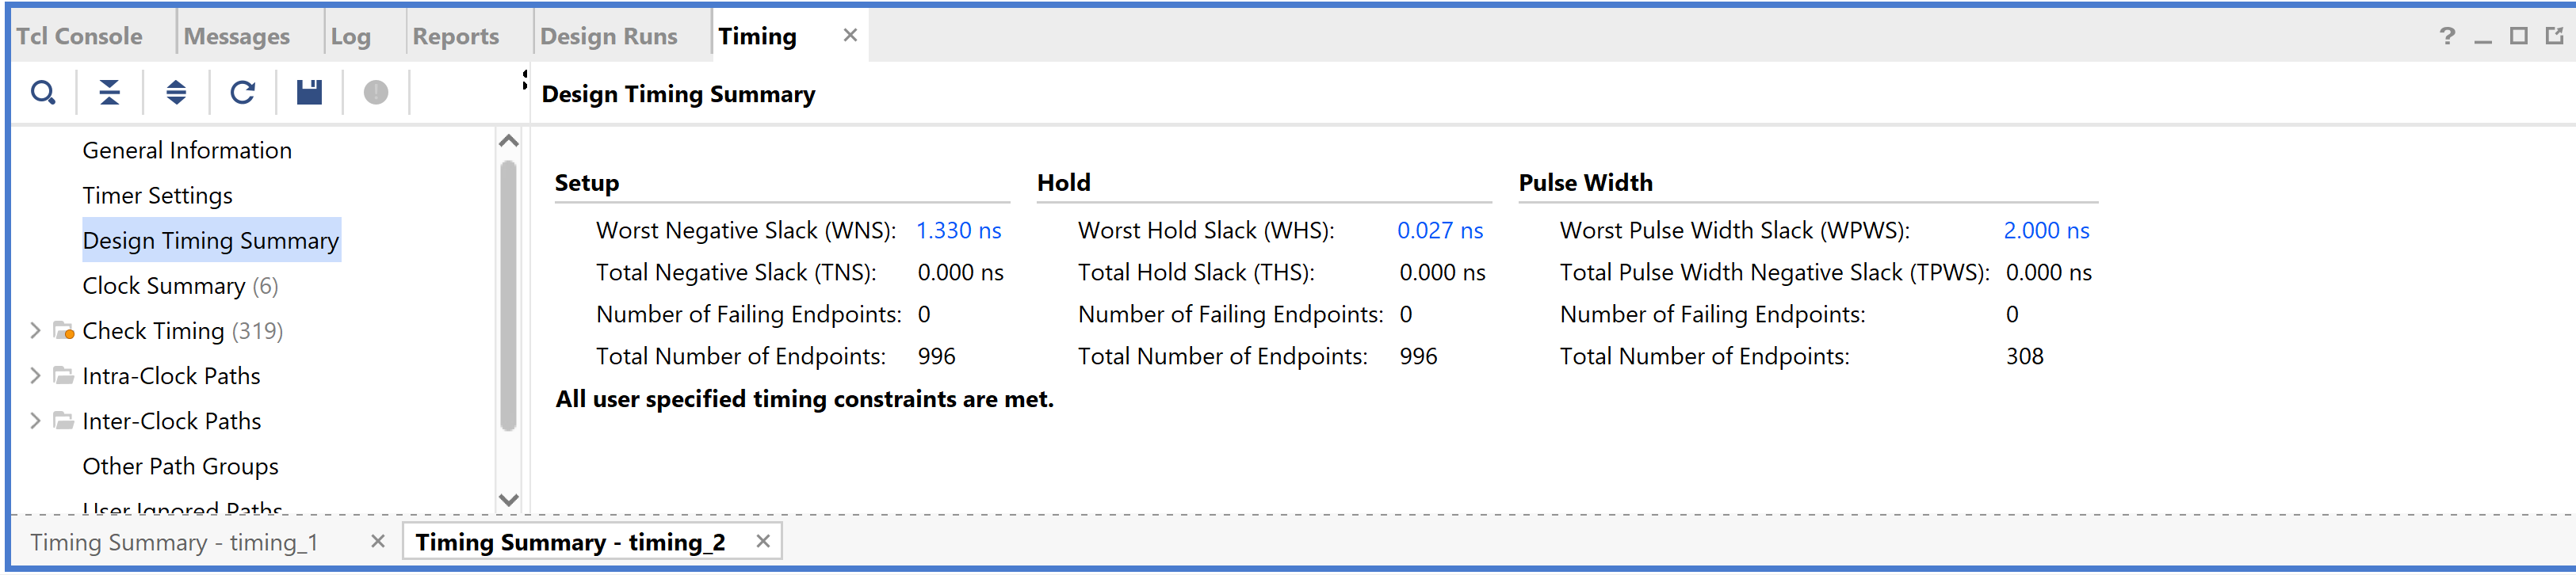
\includegraphics[width=\textwidth]{../imgs/timing_report.PNG}
        \end{figure}
    \end{alertblock}
\end{frame}

\subsection{Data throughput}
\begin{frame}
    \frametitle{Animation}
    \framesubtitle{Data throughput}
    The time of the mandelbrot generator $T_M$ depends on the resolution $R$. The time for $N$ frames is $T_F$
    \begin{equation}
        \begin{split}
            T_N&= \frac{N(1024 + 24 + 136 + 144)(768 + 3 + 6 + 29)}{75MHz}\approx\frac{N}{75}[s]\\
            T_M &=   \frac{R(257\cdot192)}{75Mhz}\approx\frac{50R}{75E3}[s]\\
            \Rightarrow R &\approx \frac{1000}{50}N = 20N
        \end{split}
    \end{equation}
    Above $T_M$ is worst case. Assuming that at most $0.5$ of the screen needs 200 iterations, we can tweak the resolution
    \begin{equation}
        R \approx 40N
    \end{equation}
\end{frame}

\subsection{Fighting the architecture}
\begin{frame}
    \frametitle{Animation}
    \framesubtitle{Fighting the architecture}
    \begin{block}{Problems encountered}
        \begin{itemize}
            \item Limited fixed point precision without pipelining
            \item Limited resolution because of iterative architecture (inhibits pipelining)
            \item Resolution prohibits pipelining in iteration block
        \end{itemize}
    \end{block}

    \begin{exampleblock}{Lesson learned}
        Before choosing an architecture
        \begin{itemize}
            \item flesh out what the plan is
            \item determine requirements and potential problems
            \item Evaluate pros and cons depending on requirements and risk analysis
        \end{itemize}
    \end{exampleblock}

\end{frame}

\end{document}